\documentclass[11pt]{article}
\usepackage{amsmath, amssymb, physics, mathtools, bm}
\usepackage{tikz, pgfplots}
\pgfplotsset{compat=1.18}
\usepackage[margin=2.3cm]{geometry}
\usepackage{siunitx, booktabs, hyperref}
\usepackage{braket}

\newcommand{\D}{\mathrm{D}}
\newcommand{\de}{\mathrm{d}}
\newcommand{\pd}[2]{\frac{\partial #1}{\partial #2}}
\newcommand{\pdd}[2]{\frac{\partial^{2} #1}{\partial #2^{2}}}

\title{B6 Condensed-Matter Physics --- Model Solutions, 2016}
\author{}
\date{}

\begin{document}
\maketitle

%==============================================================
\section*{Question 1 --- X-ray diffraction, structure factor, compressibility}

\textbf{Problem.} Define structure factor and atomic form factor; sketch $f_j(\theta)$; relate intensity to $F(hkl)$. Treat CsCl, then Fe (BCC). Derive the pressure-shift formula $(\de\theta/\de p)_T = \alpha\kappa\tan\theta$ for an Fe sample and compute $2\theta_{110}$ at ambient and at \SI{100}{GPa}.

\subsection*{(a) Structure factor and form factor}

Structure factor for the $hkl$ reflection:
\begin{equation}
F(hkl) = \sum_{j\in\text{basis}} f_j\,\exp\!\bigl[2\pi i(hx_j + ky_j + lz_j)\bigr].
\label{eq:F}
\end{equation}

The atomic form factor $f_j(\bm Q)$ is the Fourier transform of the electron density of atom $j$. Forward scattering: all electrons scatter in phase, so $f_j(\theta=0) = Z_j$. As $\theta$ grows the scatterers within the atom de-phase and $f_j$ falls.

\begin{center}
\begin{tikzpicture}[>=stealth, scale=1.0]
  \draw[->] (0,0) -- (6.5,0) node[right] {$\sin\theta/\lambda$};
  \draw[->] (0,0) -- (0,4.2) node[above] {$f_j$};
  \node[circle,fill,inner sep=1.2pt,label=left:{$Z_j$}] (Z) at (0,3.5) {};
  \draw[thick,blue] plot[domain=0:6, samples=80] (\x, {3.5*exp(-0.35*\x*\x)});
  \draw[thick,red,dashed] plot[domain=0:6, samples=80] (\x, {2.0*exp(-0.45*\x*\x)});
  \node[blue] at (4.3,1.5) {heavy};
  \node[red] at (3.0,0.5) {light};
\end{tikzpicture}
\end{center}

Diffracted intensity:
\[
I(hkl) \propto |F(hkl)|^2.
\]

\subsection*{(b) CsCl and the Fe analogue}

CsCl basis: Cs$^+$ at $(0,0,0)$ with form factor $f_\text{Cs}$; Cl$^-$ at $(\tfrac12,\tfrac12,\tfrac12)$ with $f_\text{Cl}$.

Apply \eqref{eq:F}:
\[
F(hkl) = f_\text{Cs} + f_\text{Cl}\,e^{i\pi(h+k+l)}.
\]
Use $e^{i\pi n} = (-1)^n$:
\[
F(hkl) = f_\text{Cs} + (-1)^{h+k+l}f_\text{Cl}.
\]
Square modulus:
\begin{equation}
\boxed{\;I(hkl) \propto \bigl[f_\text{Cs} + (-1)^{h+k+l}f_\text{Cl}\bigr]^2\;}
\end{equation}

Replace both ions by Fe ($f_\text{Cs},f_\text{Cl}\to f_\text{Fe}$):
\[
F(hkl) = f_\text{Fe}\bigl[1+(-1)^{h+k+l}\bigr].
\]
Square:
\[
I(hkl) \propto f_\text{Fe}^2\bigl[1+(-1)^{h+k+l}\bigr]^2 = \begin{cases} 4f_\text{Fe}^2 & h+k+l \text{ even}\\ 0 & h+k+l \text{ odd}\end{cases}.
\]

For the (111) reflection, $h+k+l=3$ (odd):
\[
I_\text{CsCl}(111) \propto (f_\text{Cs}-f_\text{Cl})^2,\qquad I_\text{Fe}(111) = 0.
\]
The (111) reflection is allowed for CsCl but \emph{systematically absent} for the Fe-substituted crystal.

The Fe structure (simple cubic with identical atoms at $0$ and $\tfrac12\tfrac12\tfrac12$) is body-centred cubic (BCC); allowed reflections satisfy $h+k+l$ even.

\subsection*{(c) Pressure dependence of $\theta$}

Bragg's law for cubic lattice:
\begin{equation}
\lambda = 2d_{hkl}\sin\theta,\qquad d_{hkl} = \frac{a}{\sqrt{h^2+k^2+l^2}}.
\label{eq:Bragg}
\end{equation}
Combine:
\[
\sin\theta = \frac{\lambda\sqrt{h^2+k^2+l^2}}{2a}.
\]
Take logarithmic derivative at fixed $\lambda$:
\[
\frac{\de\sin\theta}{\sin\theta} = -\frac{\de a}{a}.
\]
Use $\de\sin\theta = \cos\theta\,\de\theta$:
\[
\cot\theta\,\de\theta = -\frac{\de a}{a}.
\]
Volume--lattice relation: $V = a^3$, so $\de V/V = 3\,\de a/a$:
\[
\frac{\de a}{a} = \tfrac{1}{3}\frac{\de V}{V}.
\]
Definition of isothermal compressibility:
\[
\kappa = -\frac{1}{V}\!\left(\pd{V}{p}\right)_T.
\]
At fixed $T$:
\[
\frac{1}{a}\!\left(\pd{a}{p}\right)_T = -\tfrac{1}{3}\kappa.
\]
Substitute into $\cot\theta\,\de\theta = -\de a/a$:
\[
\cot\theta\!\left(\pd{\theta}{p}\right)_T = \tfrac{1}{3}\kappa.
\]
Rearrange:
\begin{equation}
\boxed{\;\!\left(\pd{\theta}{p}\right)_T = \tfrac{1}{3}\kappa\tan\theta,\qquad \alpha = \tfrac{1}{3}.\;}
\end{equation}

\subsection*{(d) Numerical evaluation}

Data: $a_0 = \SI{0.287}{nm}$, $\lambda = \SI{0.154}{nm}$, $\kappa = \SI{0.0059}{GPa^{-1}}$, $hkl = 110$ so $\sqrt{h^2+k^2+l^2}=\sqrt 2$.

\paragraph{(i) Ambient pressure.}

Apply \eqref{eq:Bragg}:
\[
\sin\theta_0 = \frac{\lambda\sqrt{2}}{2a_0} = \frac{0.154\times 1.4142}{2\times 0.287}.
\]
Numerator:
\[
0.154\times 1.4142 = 0.2178.
\]
Divide:
\[
\sin\theta_0 = \frac{0.2178}{0.574} = 0.3795.
\]
Invert:
\[
\theta_0 = \arcsin(0.3795) = 22.30^\circ.
\]
\[
\boxed{\;2\theta_0 = 44.6^\circ.\;}
\]

\paragraph{(ii) Pressure $p = \SI{100}{GPa}$.}

Lattice contraction (linearised, treating $\kappa$ constant):
\[
\frac{\Delta a}{a_0} = -\tfrac{1}{3}\kappa\,\Delta p.
\]
Numerical:
\[
\frac{\Delta a}{a_0} = -\tfrac{1}{3}\times 0.0059\times 100 = -0.1967.
\]
New lattice constant:
\[
a = a_0(1+\Delta a/a_0) = 0.287\times(1-0.1967) = \SI{0.2305}{nm}.
\]
Apply \eqref{eq:Bragg} at the new $a$:
\[
\sin\theta = \frac{\lambda\sqrt 2}{2a} = \frac{0.2178}{0.4610} = 0.4724.
\]
Invert:
\[
\theta = \arcsin(0.4724) = 28.20^\circ.
\]
\[
\boxed{\;2\theta = 56.4^\circ.\;}
\]

(The linearised approximation $\Delta a/a = -\tfrac13\kappa\Delta p$ over-estimates the contraction at \SI{100}{GPa}; the answer is reliable to $\sim 1^\circ$.)

%==============================================================
\section*{Question 2 --- Free-electron model in $d$ dimensions}

\textbf{Problem.} Define the free-electron model, Fermi energy and Fermi temperature; explain the room-temperature feel of metals. Derive $E_F$ and $g(E_F)$ in $d=1,2,3$, finding $a_d,b_d$. Estimate $E_F,T_F,\tau,\ell$ for Al and a 2D electron gas.

\subsection*{(a) Definitions and qualitative answer}

\emph{Free-electron model:} valence electrons treated as a gas of non-interacting fermions of mass $m$ moving in a flat potential, confined to volume $V=L^d$ with periodic boundary conditions; lattice ions provide only neutralising background.

\emph{Fermi energy} $E_F$: energy of the highest occupied single-particle state at $T=0$.

\emph{Fermi temperature} $T_F = E_F/k_B$: the temperature at which $k_B T$ becomes comparable to $E_F$.

For typical metals $n\sim\SI{e29}{m^{-3}}$ gives $E_F\sim\SI{5}{eV}$ and $T_F\sim\SI{e4}{K}\gg \SI{300}{K}$. Cold-to-touch sensation arises from the \emph{lattice} (phonon) heat capacity and the high electronic thermal conductivity transporting heat from the skin; the electronic heat capacity is $\sim T/T_F\ll 1$ of the classical value, but the phonon contribution at room temperature is the dominant thermal reservoir, and conduction electrons rapidly remove thermal energy from the skin.

\subsection*{(b) Fermi energy and density of states in $d$ dimensions}

Allowed $\bm k$ states have density $V/(2\pi)^d$ with spin-degeneracy $g_s=2$.

Fill a Fermi sphere of radius $k_F$:
\[
N = 2\cdot\frac{V}{(2\pi)^d}\cdot\Omega_d k_F^d / d,
\]
where $\Omega_d k_F^{d-1}$ is the surface area of a $d$-sphere of radius $k_F$ ($\Omega_1=2$, $\Omega_2=2\pi$, $\Omega_3=4\pi$); $\Omega_d k_F^d/d$ is its volume.

Solve for $k_F^d$:
\[
k_F^d = \frac{d(2\pi)^d}{2\Omega_d}\,n.
\]
Use $E_F = \hbar^2 k_F^2/(2m)$, hence $k_F^2 = (k_F^d)^{2/d}$:
\begin{equation}
\boxed{\;E_F = \frac{\hbar^2}{2m}\!\left(\frac{d(2\pi)^d}{2\Omega_d}\right)^{\!2/d}\!n^{2/d} = \frac{\hbar^2}{2m}(n a_d)^{2/d}.\;}
\end{equation}
Read off $a_d = d(2\pi)^d/(2\Omega_d)$:

\noindent
$d=1$: $a_1 = 1\cdot 2\pi /(2\cdot 2) = \pi/2$.\\
$d=2$: $a_2 = 2(2\pi)^2/(2\cdot 2\pi) = 2\pi$.\\
$d=3$: $a_3 = 3(2\pi)^3/(2\cdot 4\pi) = 3\pi^2$.

\medskip
Density of states per unit volume: count states with $E'<E$, then differentiate.

Use $N(E)/V = (2/\Omega_d')\cdot(\Omega_d/d)\cdot k(E)^d/(2\pi)^d\cdot 2$ -- equivalently, recall that
\[
N(E_F) = N \;\Rightarrow\; n = \frac{2\Omega_d}{d(2\pi)^d}k_F^d.
\]
For arbitrary $E$:
\[
\frac{N(E)}{V} = \frac{2\Omega_d}{d(2\pi)^d}k(E)^d,\qquad k(E)=\sqrt{2mE}/\hbar.
\]
Differentiate w.r.t. $E$ to obtain $g(E) = \de(N/V)/\de E$:
\[
g(E) = \frac{2\Omega_d}{d(2\pi)^d}\,d\,k^{d-1}\,\frac{\de k}{\de E} = \frac{2\Omega_d}{(2\pi)^d}\,k^{d-1}\,\frac{\de k}{\de E}.
\]
Use $\de k/\de E = m/(\hbar^2 k)$:
\[
g(E) = \frac{2\Omega_d}{(2\pi)^d}\,\frac{m\,k^{d-2}}{\hbar^2}.
\]
Evaluate at $E_F$ and divide by $n$:
\[
\frac{g(E_F)}{n} = \frac{2\Omega_d}{(2\pi)^d}\frac{m k_F^{d-2}}{\hbar^2}\cdot\frac{d(2\pi)^d}{2\Omega_d k_F^d} = \frac{d m}{\hbar^2 k_F^2} = \frac{d}{2 E_F}.
\]
Hence
\begin{equation}
\boxed{\;g(E_F) = \frac{d}{2}\,\frac{n}{E_F},\qquad b_d = d/2.\;}
\end{equation}
So $b_1 = \tfrac12$, $b_2 = 1$, $b_3 = \tfrac32$.

\subsection*{(c) Aluminium}

FCC, 4 atoms per conventional cell, valence 3 $\Rightarrow$ 12 electrons per cell of side $a=\SI{0.405}{nm}$.

Electron density:
\[
n = \frac{12}{a^3} = \frac{12}{(0.405\times 10^{-9})^3}.
\]
Cube the lattice constant:
\[
a^3 = 6.64\times 10^{-29}\,\si{m^3}.
\]
Divide:
\[
n = \frac{12}{6.64\times 10^{-29}} = 1.81\times 10^{29}\,\si{m^{-3}}.
\]

Fermi wavevector ($d=3$, $a_3=3\pi^2$):
\[
k_F = (3\pi^2 n)^{1/3} = (3\pi^2\times 1.81\times 10^{29})^{1/3}.
\]
Argument:
\[
3\pi^2\times 1.81\times 10^{29} = 5.36\times 10^{30}\,\si{m^{-3}}.
\]
Cube root:
\[
k_F = 1.75\times 10^{10}\,\si{m^{-1}}.
\]
Fermi energy:
\[
E_F = \frac{\hbar^2 k_F^2}{2m_e} = \frac{(1.055\times 10^{-34})^2(1.75\times 10^{10})^2}{2\times 9.11\times 10^{-31}}.
\]
Numerator:
\[
(1.055\times 10^{-34})^2 = 1.113\times 10^{-68},\quad (1.75\times 10^{10})^2 = 3.06\times 10^{20}.
\]
Multiply:
\[
1.113\times 10^{-68}\times 3.06\times 10^{20} = 3.41\times 10^{-48}.
\]
Divide:
\[
E_F = \frac{3.41\times 10^{-48}}{1.822\times 10^{-30}} = 1.87\times 10^{-18}\,\si{J} = \boxed{\;\SI{11.7}{eV}\;}.
\]
Fermi temperature:
\[
T_F = E_F/k_B = 1.87\times 10^{-18}/1.381\times 10^{-23} = \boxed{\;\SI{1.36e5}{K}\;}.
\]

Fermi velocity:
\[
v_F = \hbar k_F/m_e = 1.055\times 10^{-34}\times 1.75\times 10^{10}/9.11\times 10^{-31} = 2.03\times 10^{6}\,\si{m\,s^{-1}}.
\]

Drude scattering time from $\rho = m_e/(ne^2\tau)$:
\[
\tau = \frac{m_e}{n e^2 \rho} = \frac{9.11\times 10^{-31}}{1.81\times 10^{29}\times (1.602\times 10^{-19})^2\times 2.8\times 10^{-8}}.
\]
Denominator:
\[
1.81\times 10^{29}\times 2.566\times 10^{-38} = 4.64\times 10^{-9},\quad \times 2.8\times 10^{-8}=1.30\times 10^{-16}.
\]
Divide:
\[
\tau = \frac{9.11\times 10^{-31}}{1.30\times 10^{-16}} = \boxed{\;\SI{7.0e-15}{s}\;}.
\]

Mean free path:
\[
\ell = v_F\tau = 2.03\times 10^6\times 7.0\times 10^{-15} = \boxed{\;\SI{14}{nm}\;}.
\]

\subsection*{(d) 2D electron gas}

$n_{2D} = 3\times 10^{15}\,\si{m^{-2}}$, $\rho_{2D} = \SI{e3}{\Omega}$ (per square).

Fermi wavevector ($d=2$, $a_2=2\pi$):
\[
k_F = \sqrt{2\pi n_{2D}} = \sqrt{2\pi\times 3\times 10^{15}}.
\]
Argument:
\[
2\pi\times 3\times 10^{15} = 1.885\times 10^{16}.
\]
Square root:
\[
k_F = 1.37\times 10^{8}\,\si{m^{-1}}.
\]
Fermi energy:
\[
E_F = \frac{\hbar^2 k_F^2}{2m_e} = \frac{1.113\times 10^{-68}\times (1.37\times 10^8)^2}{1.822\times 10^{-30}}.
\]
Square:
\[
(1.37\times 10^8)^2 = 1.876\times 10^{16}.
\]
Numerator:
\[
1.113\times 10^{-68}\times 1.876\times 10^{16} = 2.09\times 10^{-52}.
\]
Divide:
\[
E_F = \frac{2.09\times 10^{-52}}{1.822\times 10^{-30}} = 1.15\times 10^{-22}\,\si{J} = \boxed{\;\SI{7.2e-4}{eV}\;}.
\]
(Free electron mass assumed; in a real GaAs 2DEG $m^*\approx 0.067 m_e$ would raise this $\sim15\times$.)

Fermi temperature:
\[
T_F = 1.15\times 10^{-22}/1.381\times 10^{-23} = \boxed{\;\SI{8.3}{K}\;}.
\]

Fermi velocity:
\[
v_F = \hbar k_F/m_e = 1.055\times 10^{-34}\times 1.37\times 10^8/9.11\times 10^{-31} = 1.59\times 10^4\,\si{m\,s^{-1}}.
\]

Drude in 2D: $\sigma_{2D} = n_{2D} e^2 \tau/m_e$, so $\rho_{2D} = m_e/(n_{2D} e^2 \tau)$:
\[
\tau = \frac{m_e}{n_{2D} e^2 \rho_{2D}} = \frac{9.11\times 10^{-31}}{3\times 10^{15}\times 2.566\times 10^{-38}\times 10^3}.
\]
Denominator:
\[
3\times 10^{15}\times 2.566\times 10^{-38} = 7.70\times 10^{-23},\;\times 10^3 = 7.70\times 10^{-20}.
\]
Divide:
\[
\tau = \frac{9.11\times 10^{-31}}{7.70\times 10^{-20}} = \boxed{\;\SI{1.2e-11}{s}\;}.
\]

Mean free path:
\[
\ell = v_F\tau = 1.59\times 10^4\times 1.2\times 10^{-11} = \boxed{\;\SI{0.19}{\micro m}\;}.
\]

%==============================================================
\section*{Question 3 --- Spin-$\tfrac12$ paramagnet and CuSO$_4\cdot$5H$_2$O}

\textbf{Problem.} Derive $M = M_s\tanh(\eta B/T)$ and $\chi$. Apply Hund's rules to Cu$^{2+}$, explain the role of the lattice and contrast with elemental Cu, then evaluate $\chi$ and the alignment fraction at \SI{300}{K} and \SI{2}{K} for $B=\SI{0.05}{T}$ and $\SI{5}{T}$.

\subsection*{(a) Magnetization and susceptibility}

Two-level Zeeman system: energies $\mp\tfrac12 g\mu_B B$ for $S_z = \pm\tfrac12$ ($g\simeq 2$).

Boltzmann populations:
\[
P_\pm = \frac{e^{\pm g\mu_B B/(2 k_B T)}}{Z},\qquad Z = 2\cosh\!\left(\frac{g\mu_B B}{2 k_B T}\right).
\]
Magnetic moment per spin (along $\bm B$):
\[
\langle\mu_z\rangle = \tfrac12 g\mu_B(P_+-P_-).
\]
Substitute the populations:
\[
\langle\mu_z\rangle = \tfrac12 g\mu_B\,\frac{e^{x}-e^{-x}}{e^{x}+e^{-x}},\qquad x = \frac{g\mu_B B}{2 k_B T}.
\]
Recognise hyperbolic tangent:
\[
\langle\mu_z\rangle = \tfrac12 g\mu_B\tanh x.
\]
Multiply by number density $N/V$:
\begin{equation}
\boxed{\;M = M_s\tanh(\eta B/T),\qquad M_s = \frac{N g\mu_B}{2V},\;\; \eta = \frac{g\mu_B}{2 k_B}.\;}
\label{eq:M-tanh}
\end{equation}

Small-field susceptibility: linearise $\tanh x\approx x$ for $\eta B/T\ll 1$:
\[
M \approx M_s\,\frac{\eta B}{T} = \frac{N g\mu_B}{2V}\cdot\frac{g\mu_B B}{2 k_B T}.
\]
Use $\chi = \mu_0 M/B$ (SI volume susceptibility):
\begin{equation}
\boxed{\;\chi = \frac{\mu_0 N g^2 \mu_B^2}{4 V k_B T} = \frac{\mu_0 n}{k_B T}(\tfrac12 g\mu_B)^2.\;}
\label{eq:chi}
\end{equation}
This is Curie's law $\chi\propto 1/T$.

\subsection*{(b) Cu$^{2+}$ Hund's-rule moment}

Cu$^{2+}$ configuration $3d^9$: one hole in the $3d$ shell.

Hund's rules on the hole: $S=\tfrac12$, $L=2$, $J=L+S=\tfrac52$ (more-than-half-filled shell).

Free-ion Land\'e $g$-factor:
\[
g_J = \tfrac32 + \frac{S(S+1)-L(L+1)}{2 J(J+1)} = \tfrac32 + \frac{0.75 - 6}{2\cdot 8.75} = \tfrac32 - 0.300 = 1.20.
\]
Effective Bohr-magneton number:
\[
p = g_J\sqrt{J(J+1)} = 1.20\sqrt{8.75} = 3.55.
\]
\[
\boxed{\;\mu_\text{eff}^\text{free} = 3.55\,\mu_B\;\text{(free ion, full $J$)}.\;}
\]

In the crystal the orbital moment is \emph{quenched} by the cubic/octahedral ligand field: $\langle L_z\rangle = 0$. Only spin contributes, $g\to 2$, $S=\tfrac12$:
\[
\boxed{\;p_\text{spin} = 2\sqrt{S(S+1)} = 2\sqrt{0.75} = 1.73,\;\mu_\text{eff} = 1.73\,\mu_B.\;}
\]

The SO$_4$ groups and water of hydration physically separate Cu$^{2+}$ ions, suppressing direct $d$-orbital overlap and exchange. Cu$^{2+}$ moments are therefore non-interacting paramagnetic centres rather than ordering magnetically.

Pure elemental Cu has configuration $3d^{10}4s^1$: filled $d$-shell (no net moment) plus a delocalised $4s$ conduction band. It exhibits weak Pauli paramagnetism (overwhelmed in practice by core diamagnetism), so Cu metal is overall \emph{diamagnetic}.

\subsection*{(c) Susceptibility and alignment fraction}

Number density of Cu$^{2+}$ ions:
\[
n = \frac{N_A}{V_m} = \frac{6.022\times 10^{23}}{1.092\times 10^{-4}} = 5.515\times 10^{27}\,\si{m^{-3}}.
\]
Spin-only effective moment squared (for the susceptibility formula):
\[
g^2 S(S+1) = 4\times 0.75 = 3.
\]
Generalised Curie formula (replacing $(g\mu_B/2)^2 \to g^2 S(S+1)\mu_B^2/3$ in \eqref{eq:chi} for general $S$):
\[
\chi = \frac{\mu_0 n\,g^2 S(S+1)\mu_B^2}{3 k_B T}.
\]
Evaluate the constant prefactor:
\[
\mu_0 n g^2 S(S+1)\mu_B^2 = 4\pi\times 10^{-7}\times 5.515\times 10^{27}\times 3\times (9.274\times 10^{-24})^2.
\]
Compute step by step:
\[
(9.274\times 10^{-24})^2 = 8.602\times 10^{-47}.
\]
\[
4\pi\times 10^{-7}\times 5.515\times 10^{27} = 6.929\times 10^{21}.
\]
\[
6.929\times 10^{21}\times 3 = 2.079\times 10^{22}.
\]
\[
2.079\times 10^{22}\times 8.602\times 10^{-47} = 1.789\times 10^{-24}.
\]
Divide by $3 k_B T$:
\[
\chi(T) = \frac{1.789\times 10^{-24}}{3\times 1.381\times 10^{-23}\times T} = \frac{4.32\times 10^{-2}}{T}.
\]
At \SI{300}{K}:
\[
\boxed{\;\chi(\SI{300}{K}) = 1.44\times 10^{-4}\;}\;\text{(dimensionless, SI)}.
\]
At \SI{2}{K}:
\[
\boxed{\;\chi(\SI{2}{K}) = 2.16\times 10^{-2}.\;}
\]

\paragraph{Alignment fraction.}
For spin-$\tfrac12$ in field $B$, fraction aligned with $\bm B$ is $f = \tanh x$ with $x = g\mu_B B/(2 k_B T) = \mu_B B/(k_B T)$.

Reference scale:
\[
\frac{\mu_B}{k_B} = \frac{9.274\times 10^{-24}}{1.381\times 10^{-23}} = \SI{0.6717}{K\,T^{-1}}.
\]

\paragraph{$T=\SI{300}{K}$.}
\[
B=\SI{0.05}{T}:\; x = 0.6717\times 0.05/300 = 1.12\times 10^{-4},\;\tanh x \approx 1.12\times 10^{-4}.
\]
\[
\boxed{\;f \approx 1.1\times 10^{-4}.\;}
\]
\[
B=\SI{5}{T}:\; x = 0.6717\times 5/300 = 1.12\times 10^{-2},\;\tanh x \approx 1.12\times 10^{-2}.
\]
\[
\boxed{\;f \approx 1.1\times 10^{-2}.\;}
\]

\paragraph{$T=\SI{2}{K}$.}
\[
B=\SI{0.05}{T}:\; x = 0.6717\times 0.05/2 = 1.68\times 10^{-2},\;\tanh x \approx 1.68\times 10^{-2}.
\]
\[
\boxed{\;f \approx 1.7\times 10^{-2}.\;}
\]
\[
B=\SI{5}{T}:\; x = 0.6717\times 5/2 = 1.68,\;\tanh(1.68) = 0.933.
\]
\[
\boxed{\;f \approx 0.93\;\text{(near saturation)}.\;}
\]

%==============================================================
\section*{Question 4 --- Lattice vibrations of a 1D monatomic chain}

\textbf{Problem.} Outline experimental probes of phonons; derive the dispersion of a 1D monatomic chain; sketch $\omega(k)$, $v_g(k)$, $g(\omega)$, and $C(T)$ for $a=\SI{0.2}{nm}$, $v_s=\SI{4}{km\,s^{-1}}$.

\subsection*{(a) Experimental methods}

\begin{itemize}
\item \textbf{Inelastic neutron scattering.} Thermal neutrons ($\hbar\omega\sim$ meV, $\lambda\sim$\AA) match phonon energy and momentum scales. Energy and momentum conservation, $E_i-E_f = \hbar\omega(\bm q)$ and $\bm k_i - \bm k_f = \bm q + \bm G$, map full $\omega(\bm q)$ across the BZ on triple-axis or time-of-flight spectrometers.
\item \textbf{Inelastic X-ray scattering} (synchrotron, meV resolution): same kinematics, but photon $\omega\gg$ phonon $\omega$, so the energy transfer is a tiny fraction of the incident energy; useful for small samples (high-pressure cells).
\item \textbf{Raman scattering} (visible photons): probes optic phonons at $\bm q\approx 0$ (Stokes/anti-Stokes shift); selection rules require Raman-active modes.
\item \textbf{Infrared absorption/reflectivity}: dipole-active optical phonons ($\bm q\approx 0$); reststrahlen band identifies $\omega_{TO}$, $\omega_{LO}$.
\item \textbf{Heat capacity vs $T$} (Debye fits): integrated information on $g(\omega)$.
\end{itemize}

\subsection*{(b) Equation of motion and dispersion}

Atom $n$ at equilibrium $x_n^0 = na$, displacement $u_n(t)$. Spring force from neighbour $n+1$ proportional to extension $u_{n+1}-u_n$; from $n-1$ proportional to $u_{n-1}-u_n$.

Newton's second law:
\[
m\ddot u_n = C(u_{n+1}-u_n) + C(u_{n-1}-u_n).
\]
Group:
\[
m\ddot u_n = C(u_{n+1} - 2u_n + u_{n-1}).
\]
Plane-wave ansatz:
\[
u_n(t) = u_0\,e^{i(kna - \omega t)}.
\]
Substitute:
\[
-m\omega^2 = C(e^{ika} - 2 + e^{-ika}).
\]
Use $e^{ika}+e^{-ika} = 2\cos ka$:
\[
-m\omega^2 = 2C(\cos ka - 1).
\]
Apply $1-\cos ka = 2\sin^2(ka/2)$:
\[
m\omega^2 = 4C\sin^2(ka/2).
\]
Take positive root:
\begin{equation}
\boxed{\;\omega(k) = 2\sqrt{C/m}\,|\!\sin(ka/2)|.\;}
\label{eq:disp}
\end{equation}

\subsection*{(c) Sketches}

Long-wavelength sound speed: $\omega = v_s |k|$ for $|k|a\ll 1$, giving $v_s = a\sqrt{C/m}$. Maximum frequency:
\[
\omega_\text{max} = 2\sqrt{C/m} = 2 v_s/a = 2\times 4\times 10^3/0.2\times 10^{-9} = 4\times 10^{13}\,\si{rad\,s^{-1}}.
\]
First Brillouin zone: $k\in[-\pi/a,\pi/a]$, with $\pi/a = \SI{1.57e10}{m^{-1}}$.

\paragraph{(i) Dispersion $\omega(k)$.}
\begin{center}
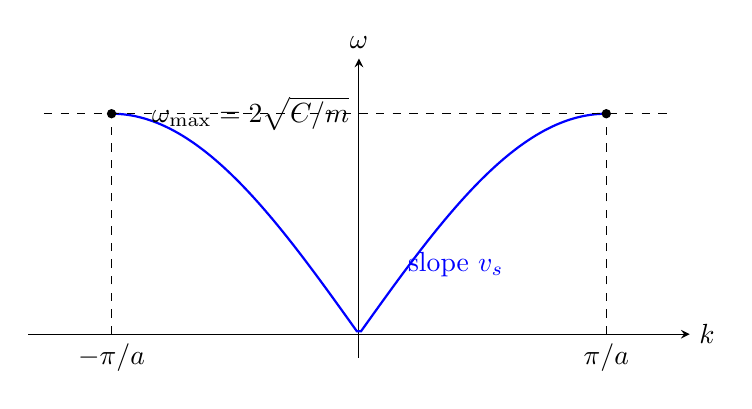
\begin{tikzpicture}[>=stealth, scale=1.0]
  \draw[->] (-4.2,0) -- (4.2,0) node[right] {$k$};
  \draw[->] (0,-0.3) -- (0,3.5) node[above] {$\omega$};
  \draw[thick,blue] plot[domain=-3.1416:3.1416, samples=120] (\x, {2.8*abs(sin(\x*0.5 r))});
  \draw[dashed] (3.1416,0) -- (3.1416,2.8);
  \draw[dashed] (-3.1416,0) -- (-3.1416,2.8);
  \draw[dashed] (-4,2.8) -- (4,2.8);
  \node[circle,fill,inner sep=1.2pt] at (3.1416,2.8) {};
  \node[circle,fill,inner sep=1.2pt] at (-3.1416,2.8) {};
  \node[below] at (3.1416,0) {$\pi/a$};
  \node[below] at (-3.1416,0) {$-\pi/a$};
  \node[left]  at (0,2.8) {$\omega_\text{max} = 2\sqrt{C/m}$};
  \node[blue,above right] at (0.5,0.6) {slope $v_s$};
\end{tikzpicture}
\end{center}

\paragraph{(ii) Group velocity $v_g(k) = \de\omega/\de k = a\sqrt{C/m}\cos(ka/2)\,\mathrm{sgn}(\sin(ka/2))$ on $|k|<\pi/a$.}

For $0<k<\pi/a$: $v_g = a\sqrt{C/m}\cos(ka/2) = v_s\cos(ka/2)$, dropping from $v_s$ at $k=0$ to $0$ at $k=\pi/a$ (and odd in $k$).

\begin{center}
\begin{tikzpicture}[>=stealth, scale=1.0]
  \draw[->] (-4.2,0) -- (4.2,0) node[right] {$k$};
  \draw[->] (0,-2.5) -- (0,2.5) node[above] {$v_g$};
  \draw[thick,red] plot[domain=0.001:3.1416, samples=80] (\x, {2*cos(\x*0.5 r)});
  \draw[thick,red] plot[domain=-3.1416:-0.001, samples=80] (\x, {-2*cos(\x*0.5 r)});
  \draw[dashed] (3.1416,0) -- (3.1416,-0.05);
  \draw[dashed] (-3.1416,0) -- (-3.1416,0.05);
  \node[circle,fill,inner sep=1.2pt] at (0,2) {};
  \node[circle,fill,inner sep=1.2pt] at (0,-2) {};
  \node[circle,fill,inner sep=1.2pt] at (3.1416,0) {};
  \node[circle,fill,inner sep=1.2pt] at (-3.1416,0) {};
  \node[left] at (0,2) {$+v_s$};
  \node[left] at (0,-2) {$-v_s$};
  \node[below] at (3.1416,0) {$\pi/a$};
  \node[below] at (-3.1416,-0.1) {$-\pi/a$};
\end{tikzpicture}
\end{center}

(Group velocity is discontinuous at $k=0$ if absolute value is taken in \eqref{eq:disp}; physically, $v_g$ changes sign through $k=0$ as drawn.)

\paragraph{(iii) Density of states $g(\omega)$.}

1D, both $\pm k$ states:
\[
g(\omega) = \frac{2}{2\pi}\,\frac{1}{|\de\omega/\de k|} = \frac{1}{\pi}\frac{1}{a\sqrt{C/m}\,|\!\cos(ka/2)|}.
\]
Use $\cos(ka/2) = \sqrt{1-\sin^2(ka/2)} = \sqrt{1 - (\omega/\omega_\text{max})^2}$:
\[
\boxed{\;g(\omega) = \frac{2}{\pi a\,\omega_\text{max}}\,\frac{1}{\sqrt{1-(\omega/\omega_\text{max})^2}},\qquad 0<\omega<\omega_\text{max}.\;}
\]
Constant low-$\omega$ value $2/(\pi a\omega_\text{max})$, van Hove divergence at $\omega_\text{max}$.

\begin{center}
\begin{tikzpicture}[>=stealth, scale=1.0]
  \draw[->] (0,0) -- (6.5,0) node[right] {$\omega$};
  \draw[->] (0,0) -- (0,3.8) node[above] {$g(\omega)$};
  \draw[thick,violet] plot[domain=0:0.99, samples=120] ({\x*5}, {1/sqrt(1-\x*\x)});
  \draw[dashed] (5,0) -- (5,3.6);
  \draw[dashed] (0,1) -- (5,1);
  \node[below] at (5,0) {$\omega_\text{max}$};
  \node[left] at (0,1) {$\frac{2}{\pi a\omega_\text{max}}$};
  \node[circle,fill,inner sep=1.2pt] at (0,1) {};
  \node[circle,fill,inner sep=1.2pt] at (5,0) {};
\end{tikzpicture}
\end{center}

\paragraph{(iv) Heat capacity $C_V(T)$.}

Low $T$ ($k_B T\ll \hbar\omega_\text{max}$): linear-dispersion phonons give 1D Debye behaviour $C_V\propto T$ (one polarization). High $T$ ($k_B T\gg \hbar\omega_\text{max}$): equipartition $C_V \to N k_B$ per atom (Dulong--Petit limit, classical).

Crossover scale: $\theta_D = \hbar\omega_\text{max}/k_B$.
\[
\theta_D = \hbar\omega_\text{max}/k_B = (1.055\times 10^{-34}\times 4\times 10^{13})/1.381\times 10^{-23} = \SI{306}{K}.
\]

\begin{center}
\begin{tikzpicture}[>=stealth, scale=1.0]
  \draw[->] (0,0) -- (6.5,0) node[right] {$T$};
  \draw[->] (0,0) -- (0,3.8) node[above] {$C_V$};
  \draw[thick,teal] plot[domain=0:6, samples=120] (\x, {3*tanh(\x*0.5)});
  \draw[dashed] (0,3) -- (6,3);
  \draw[dashed] (1.6,0) -- (1.6,3);
  \node[circle,fill,inner sep=1.2pt] at (0,0) {};
  \node[below] at (1.6,0) {$\theta_D \sim \SI{306}{K}$};
  \node[left]  at (0,3) {$N k_B$};
  \node[teal,above] at (0.6,0.3) {$\propto T$};
\end{tikzpicture}
\end{center}

\end{document}
